% Options for packages loaded elsewhere
\PassOptionsToPackage{unicode}{hyperref}
\PassOptionsToPackage{hyphens}{url}
%
\documentclass[
]{article}
\usepackage{amsmath,amssymb}
\usepackage{iftex}
\ifPDFTeX
  \usepackage[T1]{fontenc}
  \usepackage[utf8]{inputenc}
  \usepackage{textcomp} % provide euro and other symbols
\else % if luatex or xetex
  \usepackage{unicode-math} % this also loads fontspec
  \defaultfontfeatures{Scale=MatchLowercase}
  \defaultfontfeatures[\rmfamily]{Ligatures=TeX,Scale=1}
\fi
\usepackage{lmodern}
\ifPDFTeX\else
  % xetex/luatex font selection
\fi
% Use upquote if available, for straight quotes in verbatim environments
\IfFileExists{upquote.sty}{\usepackage{upquote}}{}
\IfFileExists{microtype.sty}{% use microtype if available
  \usepackage[]{microtype}
  \UseMicrotypeSet[protrusion]{basicmath} % disable protrusion for tt fonts
}{}
\makeatletter
\@ifundefined{KOMAClassName}{% if non-KOMA class
  \IfFileExists{parskip.sty}{%
    \usepackage{parskip}
  }{% else
    \setlength{\parindent}{0pt}
    \setlength{\parskip}{6pt plus 2pt minus 1pt}}
}{% if KOMA class
  \KOMAoptions{parskip=half}}
\makeatother
\usepackage{xcolor}
\usepackage[margin=1in]{geometry}
\usepackage{color}
\usepackage{fancyvrb}
\newcommand{\VerbBar}{|}
\newcommand{\VERB}{\Verb[commandchars=\\\{\}]}
\DefineVerbatimEnvironment{Highlighting}{Verbatim}{commandchars=\\\{\}}
% Add ',fontsize=\small' for more characters per line
\usepackage{framed}
\definecolor{shadecolor}{RGB}{248,248,248}
\newenvironment{Shaded}{\begin{snugshade}}{\end{snugshade}}
\newcommand{\AlertTok}[1]{\textcolor[rgb]{0.94,0.16,0.16}{#1}}
\newcommand{\AnnotationTok}[1]{\textcolor[rgb]{0.56,0.35,0.01}{\textbf{\textit{#1}}}}
\newcommand{\AttributeTok}[1]{\textcolor[rgb]{0.13,0.29,0.53}{#1}}
\newcommand{\BaseNTok}[1]{\textcolor[rgb]{0.00,0.00,0.81}{#1}}
\newcommand{\BuiltInTok}[1]{#1}
\newcommand{\CharTok}[1]{\textcolor[rgb]{0.31,0.60,0.02}{#1}}
\newcommand{\CommentTok}[1]{\textcolor[rgb]{0.56,0.35,0.01}{\textit{#1}}}
\newcommand{\CommentVarTok}[1]{\textcolor[rgb]{0.56,0.35,0.01}{\textbf{\textit{#1}}}}
\newcommand{\ConstantTok}[1]{\textcolor[rgb]{0.56,0.35,0.01}{#1}}
\newcommand{\ControlFlowTok}[1]{\textcolor[rgb]{0.13,0.29,0.53}{\textbf{#1}}}
\newcommand{\DataTypeTok}[1]{\textcolor[rgb]{0.13,0.29,0.53}{#1}}
\newcommand{\DecValTok}[1]{\textcolor[rgb]{0.00,0.00,0.81}{#1}}
\newcommand{\DocumentationTok}[1]{\textcolor[rgb]{0.56,0.35,0.01}{\textbf{\textit{#1}}}}
\newcommand{\ErrorTok}[1]{\textcolor[rgb]{0.64,0.00,0.00}{\textbf{#1}}}
\newcommand{\ExtensionTok}[1]{#1}
\newcommand{\FloatTok}[1]{\textcolor[rgb]{0.00,0.00,0.81}{#1}}
\newcommand{\FunctionTok}[1]{\textcolor[rgb]{0.13,0.29,0.53}{\textbf{#1}}}
\newcommand{\ImportTok}[1]{#1}
\newcommand{\InformationTok}[1]{\textcolor[rgb]{0.56,0.35,0.01}{\textbf{\textit{#1}}}}
\newcommand{\KeywordTok}[1]{\textcolor[rgb]{0.13,0.29,0.53}{\textbf{#1}}}
\newcommand{\NormalTok}[1]{#1}
\newcommand{\OperatorTok}[1]{\textcolor[rgb]{0.81,0.36,0.00}{\textbf{#1}}}
\newcommand{\OtherTok}[1]{\textcolor[rgb]{0.56,0.35,0.01}{#1}}
\newcommand{\PreprocessorTok}[1]{\textcolor[rgb]{0.56,0.35,0.01}{\textit{#1}}}
\newcommand{\RegionMarkerTok}[1]{#1}
\newcommand{\SpecialCharTok}[1]{\textcolor[rgb]{0.81,0.36,0.00}{\textbf{#1}}}
\newcommand{\SpecialStringTok}[1]{\textcolor[rgb]{0.31,0.60,0.02}{#1}}
\newcommand{\StringTok}[1]{\textcolor[rgb]{0.31,0.60,0.02}{#1}}
\newcommand{\VariableTok}[1]{\textcolor[rgb]{0.00,0.00,0.00}{#1}}
\newcommand{\VerbatimStringTok}[1]{\textcolor[rgb]{0.31,0.60,0.02}{#1}}
\newcommand{\WarningTok}[1]{\textcolor[rgb]{0.56,0.35,0.01}{\textbf{\textit{#1}}}}
\usepackage{graphicx}
\makeatletter
\def\maxwidth{\ifdim\Gin@nat@width>\linewidth\linewidth\else\Gin@nat@width\fi}
\def\maxheight{\ifdim\Gin@nat@height>\textheight\textheight\else\Gin@nat@height\fi}
\makeatother
% Scale images if necessary, so that they will not overflow the page
% margins by default, and it is still possible to overwrite the defaults
% using explicit options in \includegraphics[width, height, ...]{}
\setkeys{Gin}{width=\maxwidth,height=\maxheight,keepaspectratio}
% Set default figure placement to htbp
\makeatletter
\def\fps@figure{htbp}
\makeatother
\setlength{\emergencystretch}{3em} % prevent overfull lines
\providecommand{\tightlist}{%
  \setlength{\itemsep}{0pt}\setlength{\parskip}{0pt}}
\setcounter{secnumdepth}{-\maxdimen} % remove section numbering
\ifLuaTeX
  \usepackage{selnolig}  % disable illegal ligatures
\fi
\usepackage{bookmark}
\IfFileExists{xurl.sty}{\usepackage{xurl}}{} % add URL line breaks if available
\urlstyle{same}
\hypersetup{
  hidelinks,
  pdfcreator={LaTeX via pandoc}}

\author{}
\date{\vspace{-2.5em}}

\begin{document}

\section{Project Written Sections}\label{project-written-sections}

\#Introduction

\section{Background}\label{background}

\begin{Shaded}
\begin{Highlighting}[]
\FunctionTok{library}\NormalTok{(knitr)}
\end{Highlighting}
\end{Shaded}

\begin{verbatim}
## Warning: package 'knitr' was built under R version 4.4.3
\end{verbatim}

\subsection{Defining Food Insecurity}\label{defining-food-insecurity}

\begin{verbatim}
Food insecurity refers to the lack of reliable access to sufficient, nutritious food which encompasses four dimensions: availability, access, stability and utilization (Uppal, 2023). Insecure household may face difficulties in acquiring food, affording nutritious meals or maintain stable access due to infrastructure or economic disruption. According to the USDA, food insecurity can range from limited dietary variety and quality to severe disruptions like insufficient food intake (Coleman-Jensen et al., 2019). Beyond nutritional concerns, it is closely linked to a higher likelihood of chronic illnesses, mental health issues, frequent hospital visits and even mortality (Uppal, 2023). In 2018, around 11.1% of households in the United States, over 14 million, struggle with food insecurity, including 4.3% that experienced very low food security (Coleman-Jensen et al., 2019). On a global scale, rates of food insecurity have been increasing, driven by factors like inflation, economic uncertainty, and systemic inequalities. While these national statistics are alarming, Texas often exceeds national averages, particularly in marginalized and rural areas. In 2020-2022, 15.5% of households were food insecure, exceeding the national average of 12.8% (USDA ERS, 2023). Therefore, highlighting its urgency as a case study for deeper spatial and racial food access disparities (Dean & Sharkey, 20100; Janda et al., 2022). The complex and multifaceted nature of food insecurity calls for both large-scale policy reforms and locally tailored, community-driven strategies.
\end{verbatim}

\subsection{Structural Causes of Food
Insecurity}\label{structural-causes-of-food-insecurity}

Food insecurity is associated with various structural inequalities,
including income disparities, access to capital, and systemic barriers
rooted in racism. Several studies revealed that food insecurity is the
result of compounding factors that disproportionately affect racialized
communities in the United States. In a systematic review of studies on
food deserts by Beaulac et al.~(2009), they concluded that socioeconomic
deprivation at the community level intensifies individual-level
disparities in the United States. Their review concluded that low-income
neighbourhoods that were predominantly African American continuously had
fewer supermarkets while experiencing limited geographic access to
affordable, healthy food (Beaulac et al., 2009). This structural
disadvantage hinders an entire community's access to nutritious foods,
especially in areas dominated by convenience stores that typically offer
unhealthy and expensive food items.

Similarly, Myers and Painter (2017) examined the relationship between
race/ethnicity, nativity and food insecurity. They found that Black and
Latino households in the United States suffer more than twice as much
from food insecurity in comparison to white households, even when
accounting for socioeconomic status (Myers \& Painter, 2017). Given that
minority neighbourhoods have fewer quality supermarkets regardless of
socioeconomic status, the authors suggest this gap stems from spatial
inequalities. These spatial inequalities indicate that race, independent
of income, shapes access to nutritious food. Nam et al.~(2015) confirm
these findings in their analysis of racial disparities in food
insufficiency. In their study, the authors found that Black, Hispanic,
and American Indian families experience food insecurity at a
statistically significantly higher rate than White families (Nam et al.,
2015). When the authors conducted a breakdown of contributing factors,
they discovered that this disparity among the minority groups was tied
mainly to lower homeownership rates, access to credit, and insufficient
financial assets (Nam et al., 2015). These economic disparities increase
susceptibility during times of financial hardship, restricting minority
families' ability to protect themselves from food insecurity.
Collectively, the research conducted emphasizes that the intersection of
race and socioeconomic class creates compounded disadvantages for
families of non-White backgrounds. Furthermore, this suggests that food
insecurity in the United States, particularly in Texas, is not solely
tied to income but several other systemic barriers that are shaped by
racial inequality.

\subsection{Race, Place, and Access}\label{race-place-and-access}

T exas food insecurity is deeply shaped by spatial and racial
inequalities in food access. In rural Central Texas, residents often
face limited access to supermarkets and healthy food outlets, typically
traveling long distances for groceries and relying on nearby convenience
stores with fewer nutritious options. This geographic isolation, coupled
with underdeveloped infrastructure and lack of public transportation,
contributes to higher food prices and limited dietary quality compared
to urban areas (Dean \& Sharkey, n.d.; Dean \& Sharkey, 2011). Janda et
al.~(2022) further support these findings, examining food insecurities
across different geographic contexts in Travis County. They found that
individuals living in rural zip codes were more than twice as likely to
experience food insecurities compared to those in urban areas. This
remains significant even after controlling for factors like income,
educational level, employment status and access to transportation (Janda
et al., 2022). Additionally, Janda's 2020 dissertation research
documented rural and peri-urban callers to the 2-1-1 helpline in Central
Texas. The finding shows that these areas were significantly more likely
to seek help with food assistance. This was true for individuals living
in zip codes that lacked supermarkets, emphasizing the role that
geographic proximity plays in shaping spatial disparities in food
access.

Race and geography shape disparities in food insecurity across Texas.
The Supplemental Nutrition Assistance Program (SNAP), formerly known as
food stamps, was established to combat food insecurity among low-income
populations providing assistance to purchase food.Yet disparities
persist even among SNAP-eligible households. Samuel et al.~(2023) found
that across the United States, SNAP-eligible Black and multiracial
households experience higher rates of food insecurities compared to
White counterparts. This disparity was especially evident among those
who were not enrolled in the program. Among households not participating
in SNAP, those that identify entirely Black were 52\% more likely to
experience food insecurity compared to White households. Similarly,
multiracial households faced a 42\% higher risk of food insecurity than
their White counterparts. Importantly, among households actively
participating in SNAP, the racial disparities in food insecurity were no
longer observed. This suggests that while food assistance programs can
help reduce the effects of structural inequalities, it does not entirely
eliminate them (Samuel et al., 2023). In Central Texas, Janda et
al.~(2022) reported that Hispanic participants had 2.79 times greater
odds of being food insecure than participants who were non-Hispanic
white. This aligns with the broader finding identifying that
race/ethnicity often intersect with income in shaping food insecurity
risk (Janda et al., 2022). Janda and others highlight that communities
of color are disproportionately affected by systemic barriers such as
reduced access to full-service grocery stores and overreliance on small
retailers with fewer healthy options (Beaulac et al., 2009; Walker et
al., 2010; Janda et al., 2022).

Rural Texans face unique and persistent barriers to food security, often
shaped by limited infrastructure, social isolation and inadequate food
retail presence. Dean and Sharkey (2011) emphasized that rural areas not
only lack supermarkets, but exhibit weaker social networks and less
communal support. These factors further undermine resilience against
food insecurity. Janda et al.~(2022) extends on this understanding by
showing that rural residents in Central Texas often live farther from
supermarkets, an average of 1.66 miles but closer to convenience stores
with an average of 0.67 miles. This proximity gap disproportionately
affects low-income and Hispanic households, exacerbating nutritional
disparities and increasing vulnerability to food insecurity (Janda et
al., 2022).

Moreover, the uneven distribution of food retailers and limited
transportation options in rural areas indicate that effective solutions
must be customized to local needs and the resident's lived experiences.
Janda et al.~(2022), emphasize the importance of incorporating factors
such as perceived accessibility, community preferences and cultural
appropriateness. These factors are often overlooked in conventional
approaches to identify food deserts.

\subsection{Policy Landscape and
Limitations}\label{policy-landscape-and-limitations}

SNAP (formerly known as food stamps) is the largest federal food
assistance initiative in the United States. It is designed to alleviate
food insecurity by providing financial support for low-income families.
While SNAP reduces food insecurity by helping millions of families each
year, its effectiveness is still limited by structural and environmental
factors. Grummon and Taillie (2018) found that even with SNAP
participation, there are still racial disparities in purchasing
patterns. Their findings show that Black SNAP participants tended to
purchase more processed meats, sweeteners, and low-nutrient foods
compared to White participants of the program (Grummon \& Taillie,
2018). Notably, these disparities do not appear in non-participating
families. This suggests that the SNAP program, although it may aid in
access to food, does not enhance diet quality equally among different
racial/ethnic groups (Grummon \& Taillie, 2018).

Odoms-Young (2018) highlights how these disparities are influenced by
structural racism in food systems and public policy. Factors such as
housing segregation, financial inequality, and high incarceration rates
disproportionately impact communities of colour (Odoms-Young, 2018).
These factors create barriers to food assistance and healthy food
options. The author also notes that these racial disparities exist even
when socioeconomic factors are removed (Odoms-Young, 2018), highlighting
once again that race independently impacts access to nutritious foods.

A study of a low-income Latino neighbourhood in Upstate New York by
Lopez-Class and Hosler (2010) revealed that most local stores that
accepted SNAP still provided limited access to nutritious items and high
food prices. For example, only one store in the entire neighbourhood
carried high-fiber bread compared to seven in the adjacent non-Latino
neighbourhood (Lopez-Class \& Hosler, 2010). On top of this, many of the
stores were not disability-accessible and public transport to these
locations was insufficient (Lopez-Class \& Hosler, 2010). Consequently,
residents without cars were often forced to rely on smaller retailers
with higher prices and fewer nutritional options, which erodes the
intended support of SNAP assistance (Lopez-Class \& Hosler, 2010).

In conclusion, while SNAP has been critical for tackling food
insecurity, its current system fails to address the disparities in
purchasing patterns of minority groups and the system issues that lead
to these racial and geographic disparities. Effective policy reforms are
required to consider inequitable food access caused by transportation
limitations, and racial and place-based disparities that constrain how
SNAP assistance is used.

\subsection{Gaps in the Literature}\label{gaps-in-the-literature}

Despite substantial research on food insecurity in the United States,
particularly in Texas, a significant gap remains. The gaps are seen in
studies that integrate both spatial and racial/ethnic dimensions using
spatially explicit methods. Most of the existing studies focus on racial
disparities (e.g.~food insecurity among Black, Latino and immigrant
community) or spatial disparities (e.g.~rural-urban food deserts) but
rarely examine how race, place and poverty interact at a localized scale
(Beaulac et al., 2009; Myers \& Painter, 2017). Myers and Painter (2017)
found persistent food insecurity divide across racial/ethnic and
nativity lines, even after controlling for socioeconomic status. On the
other hand, spatial studies like Janda et al.~(2022) and Lopez-Class \&
Hosler (2010) underscore geographic barriers like proximity to
supermarkets but does not consistently take into account for racialized
experiences of those affected. Furthermore, studies examining the impact
on SNAP on reducing disparities have primary used cross-sectional or
nationwide datasets. This often fails to capture how SNAP participation
intersect with race and geographical context at a local level (Grummon
\& Taillie, 2018). This leaves an analytical blind spot regarding
localized, intersectional factors of food insecurity in Texas. This
project hopefully contributed to closing this gap by using inferential
and spatial statistical methods to examine how race, income, location
and SNAP usage interact, offering a greater understanding of food access
inequalities in Texas.

\section{Study Area}\label{study-area}

\section{Methods}\label{methods}

\subsection{Methods for Spatial
Statistics}\label{methods-for-spatial-statistics}

County-level data on food stamp usage and race in Texas were analyzed
using the df\_race.rds shapefile. This shapefile included variables such
as the percentage of residents receiving food stamps and racial
composition. It was imported into R and reprojected using
st\_transform() to EPSG:3857 to ensure accurate distance-based and
spatial relationship calculations.

\begin{verbatim}
To visualize the geographic distribution of food stamp usage, an initial choropleth map was created using ggplot() and geom_sf(), with the variable food_stamp_p representing the percentage of food stamp recipients in each county. The scale_fill_viridis_c() was used to apply a colour gradient that improves interpretability for viewers by emphasizing variation in values. Prior to analysis, counties with missing values were excluded using filter(!is.na(food_stamp_p)) to prevent skewed results and ensure clean spatial computations.
\end{verbatim}

To analyze local spatial interactions, a neighbourhood structure was
established using Queen contiguity through the poly2nb() function, which
identifies counties as neighbours if they share a boundary or a corner
point. This structure was then transformed into a spatial weights matrix
using nb2listw(), allowing the influence of neighbouring counties to be
incorporated into subsequent spatial analyses.

Spatial moving averages (SMAs) were computed using lag.listw() for key
variables such as food stamp usage (sma\_food\_stamp\_p) and racial
proportions (e.g., sma\_white\_p, sma\_black\_p, sma\_asian\_p,
sma\_american\_indian\_p, sma\_pacific\_islander\_p, sma\_other\_p).
SMAs provide a smoothed view of regional patterns by averaging the
values of surrounding counties instead of the raw data. This approach
emphasizes clusters of consistent low or high values, making the broader
spatial trend easy to identify.

A null simulation envelope was generated to assess whether observed
spatial patterns were stronger than would be expected under random
distribution. It involved randomizing the food stamp usage values using
a sample (food\_stamp\_p) and recalculating the SMA of the randomized
data. Therefore, it created a baseline scenario representing spatial
randomness, allowing for visual and statistical comparison with the
actual SMA pattern. The difference between the observed and randomized
results offers insight into the presence and strength of spatial
autocorrelation within the data.

\begin{verbatim}
The local Gi* statistic (Local G) was computed using localG() from the spdep package to identify areas of statistically significant clustering. This technique evaluates each county’s value relative to the average of its neighbouring counties and generates a Z-score. This Z-score determines whether it belongs to a statistically significant high-value cluster (hotspot) or a low-value cluster (coldspot). The analysis was applied to food stamp usage and racial proportion to explore the spatial overlap between race and food insecurity. The resulting Gi* values were incorporated using mutate() and converted to numeric format using as.numeric() to enable plotting. Since localG() outputs a specialized object class, converting the results to numeric format was required to ensure compatibility with ggplot() for mapping and visualization.

Lastly, maps were generated to visualize the Gi* Z-scores using ggplot() and scale_fill_gradient2(), with a midpoint of zero. Red tones indicated statistically significant hotspots (high-value clusters), blue/green tones indicated coldspots (low-value clusters), and yellow areas represented neutral or non-significant regions. This mapping approach successfully highlighted clusters of food insecurity and racial distribution, offering a spatial perspective for understanding systemic disparities among the counties in Texas. 
\end{verbatim}

\#\#Methods for Regression Analyses Regression models were estimated
using tract-level data on per-capita food stamp usage, racial
composition, and several control variables, including unemployment rate,
median household income, and per-capita households with children.

Initial analyses employed methods of Ordinary Least Squares (OLS)
regression to examine the relationship between food stamp usage and
racial composition, controlling for socioeconomic factors. To resolve
the challenge of perfect multicollinearity, the White racial category
was omitted as the reference group. Both linear and log-transformed
models were tested to explore differences in functional form. However, a
Moran's I test using the moran.test() function revealed significant
spatial dependence, prompting further investigation.

To address spatial autocorrelation in the OLS residuals, a spatial
weights matrix was constructed using a k-nearest neighbors approach.
Tract centroids were calculated using st\_centroid(), and neighborhoods
were defined with k=4 using knearneigh(). The final spatial weights
matrix was constructed using nb2listw().

A geographically weighted regression (GWR) model with Gaussian weighting
was then estimated using gwr.sel() and gwr() to produce localized
estimates. However, residuals from the GWR model remained spatially
autocorrelated, as indicated by a Moran's I test.

To explicitly account for residual spatial dependence, a Spatial Error
Model (SEM) was estimated. This method accounts for spatial
autocorrelation by incorporating a function of the spatially dependent
residuals within the error term. A Moran's I test confirmed spatial
independence of the SEM residuals, indicating the validity of the
estimates.

Moran's I = -0.0396, p-value = 3.77e-07

\#\#Regression Analyses

The Spatial Error Model (SEM) reveals statistically significant
relationships between food stamp usage and racial composition across
Texas census tracts. Because the per capita proportions for all race
groups must sum to 1.00, the White race category was excluded from the
regression to avoid multicollinearity. Therefore, ``White'' serves as
the reference group.

Holding all other variables constant, a one percent increase in the
share of Black residents corresponds to a 0.057\% rise in per capita
food stamp usage (p \textless{} 0.0001), while a one percent increase in
the ``other'' category yields a 0.037\% increase (p \textless{} 0.0001).
In contrast, a one percent uptick in the Asian share leads to a 0.018\%
decrease in food stamp usage (p ≈ 0.007). The American Indian and
Pacific Islander coefficients are not statistically significant at the
10\% level (p = 0.603 and p = 0.198, respectively).

Among the control variables, every additional \$10,000 in median
household income predicts about a 0.006\% decrease in per capita food
stamp usage (p \textless{} 0.0001). On the other hand, higher values in
per-capita households with children and unemployment rate increase
reliance on food stamps by 0.197\% and 0.133\% respectively (both p
\textless{} 0.0001). The SEM's spatial error coefficient is λ = 0.53 (p
\textless{} 0.001), indicating substantial spatial clustering in the
regression errors. This high lambda value justifies our use of the SEM
specification. Indeed, the SEM outperforms OLS with a much lower AIC
(--26,092 vs.~--24,818). To confirm that we've successfully removed
residual spatial autocorrelation, we ran a Moran's I test on the SEM
residuals. The result of Moran's I = --0.0396 (p \textless{} 0.0001)
reveals a slight negative autocorrelation that is highly significant.
This demonstrates that the SEM specification has absorbed spatial
dependence in the residuals, thus validating the reliability of our
regression coefficients.

Together, these results reveal a strong relationship between race and
food stamp usage across Texas census tracts. Relative to the White
population (which serves as the reference group), areas with a higher
proportion of Black residents show the largest increase in food stamp
usage. Therefore, communities with a high percentage of Black residents
experience a disproportionately larger reliance on SNAP compared to any
other race group. Similarly, tracts with a greater share of residents
classified in the ``other'' racial category also show higher food stamp
usage than White census tracts, though this relationship is slightly
weaker than it is for Black communities. In contrast, tracts with a
greater proportion of Asian residents actually show lower food stamp
usage compared to White tracts. The coefficients for American Indian and
Pacific Islander groups are not statistically significant, and so these
coefficients are not directly interpretable. Additionally, the control
variables follow expected patterns. A higher median household income is
associated with lower food stamp use, while greater unemployment and a
greater share of households with children correspond with increased food
stamp usage.

\begin{verbatim}
Moran I test under randomisation
\end{verbatim}

data: model.sem1\$residuals\\
weights: df\_race\_c.w

Moran I statistic standard deviate = -4.947, p-value = 3.769e-07
alternative hypothesis: less sample estimates: Moran I statistic
Expectation Variance -3.960006e-02 -1.471670e-04 6.360299e-05

\begin{figure}
\centering
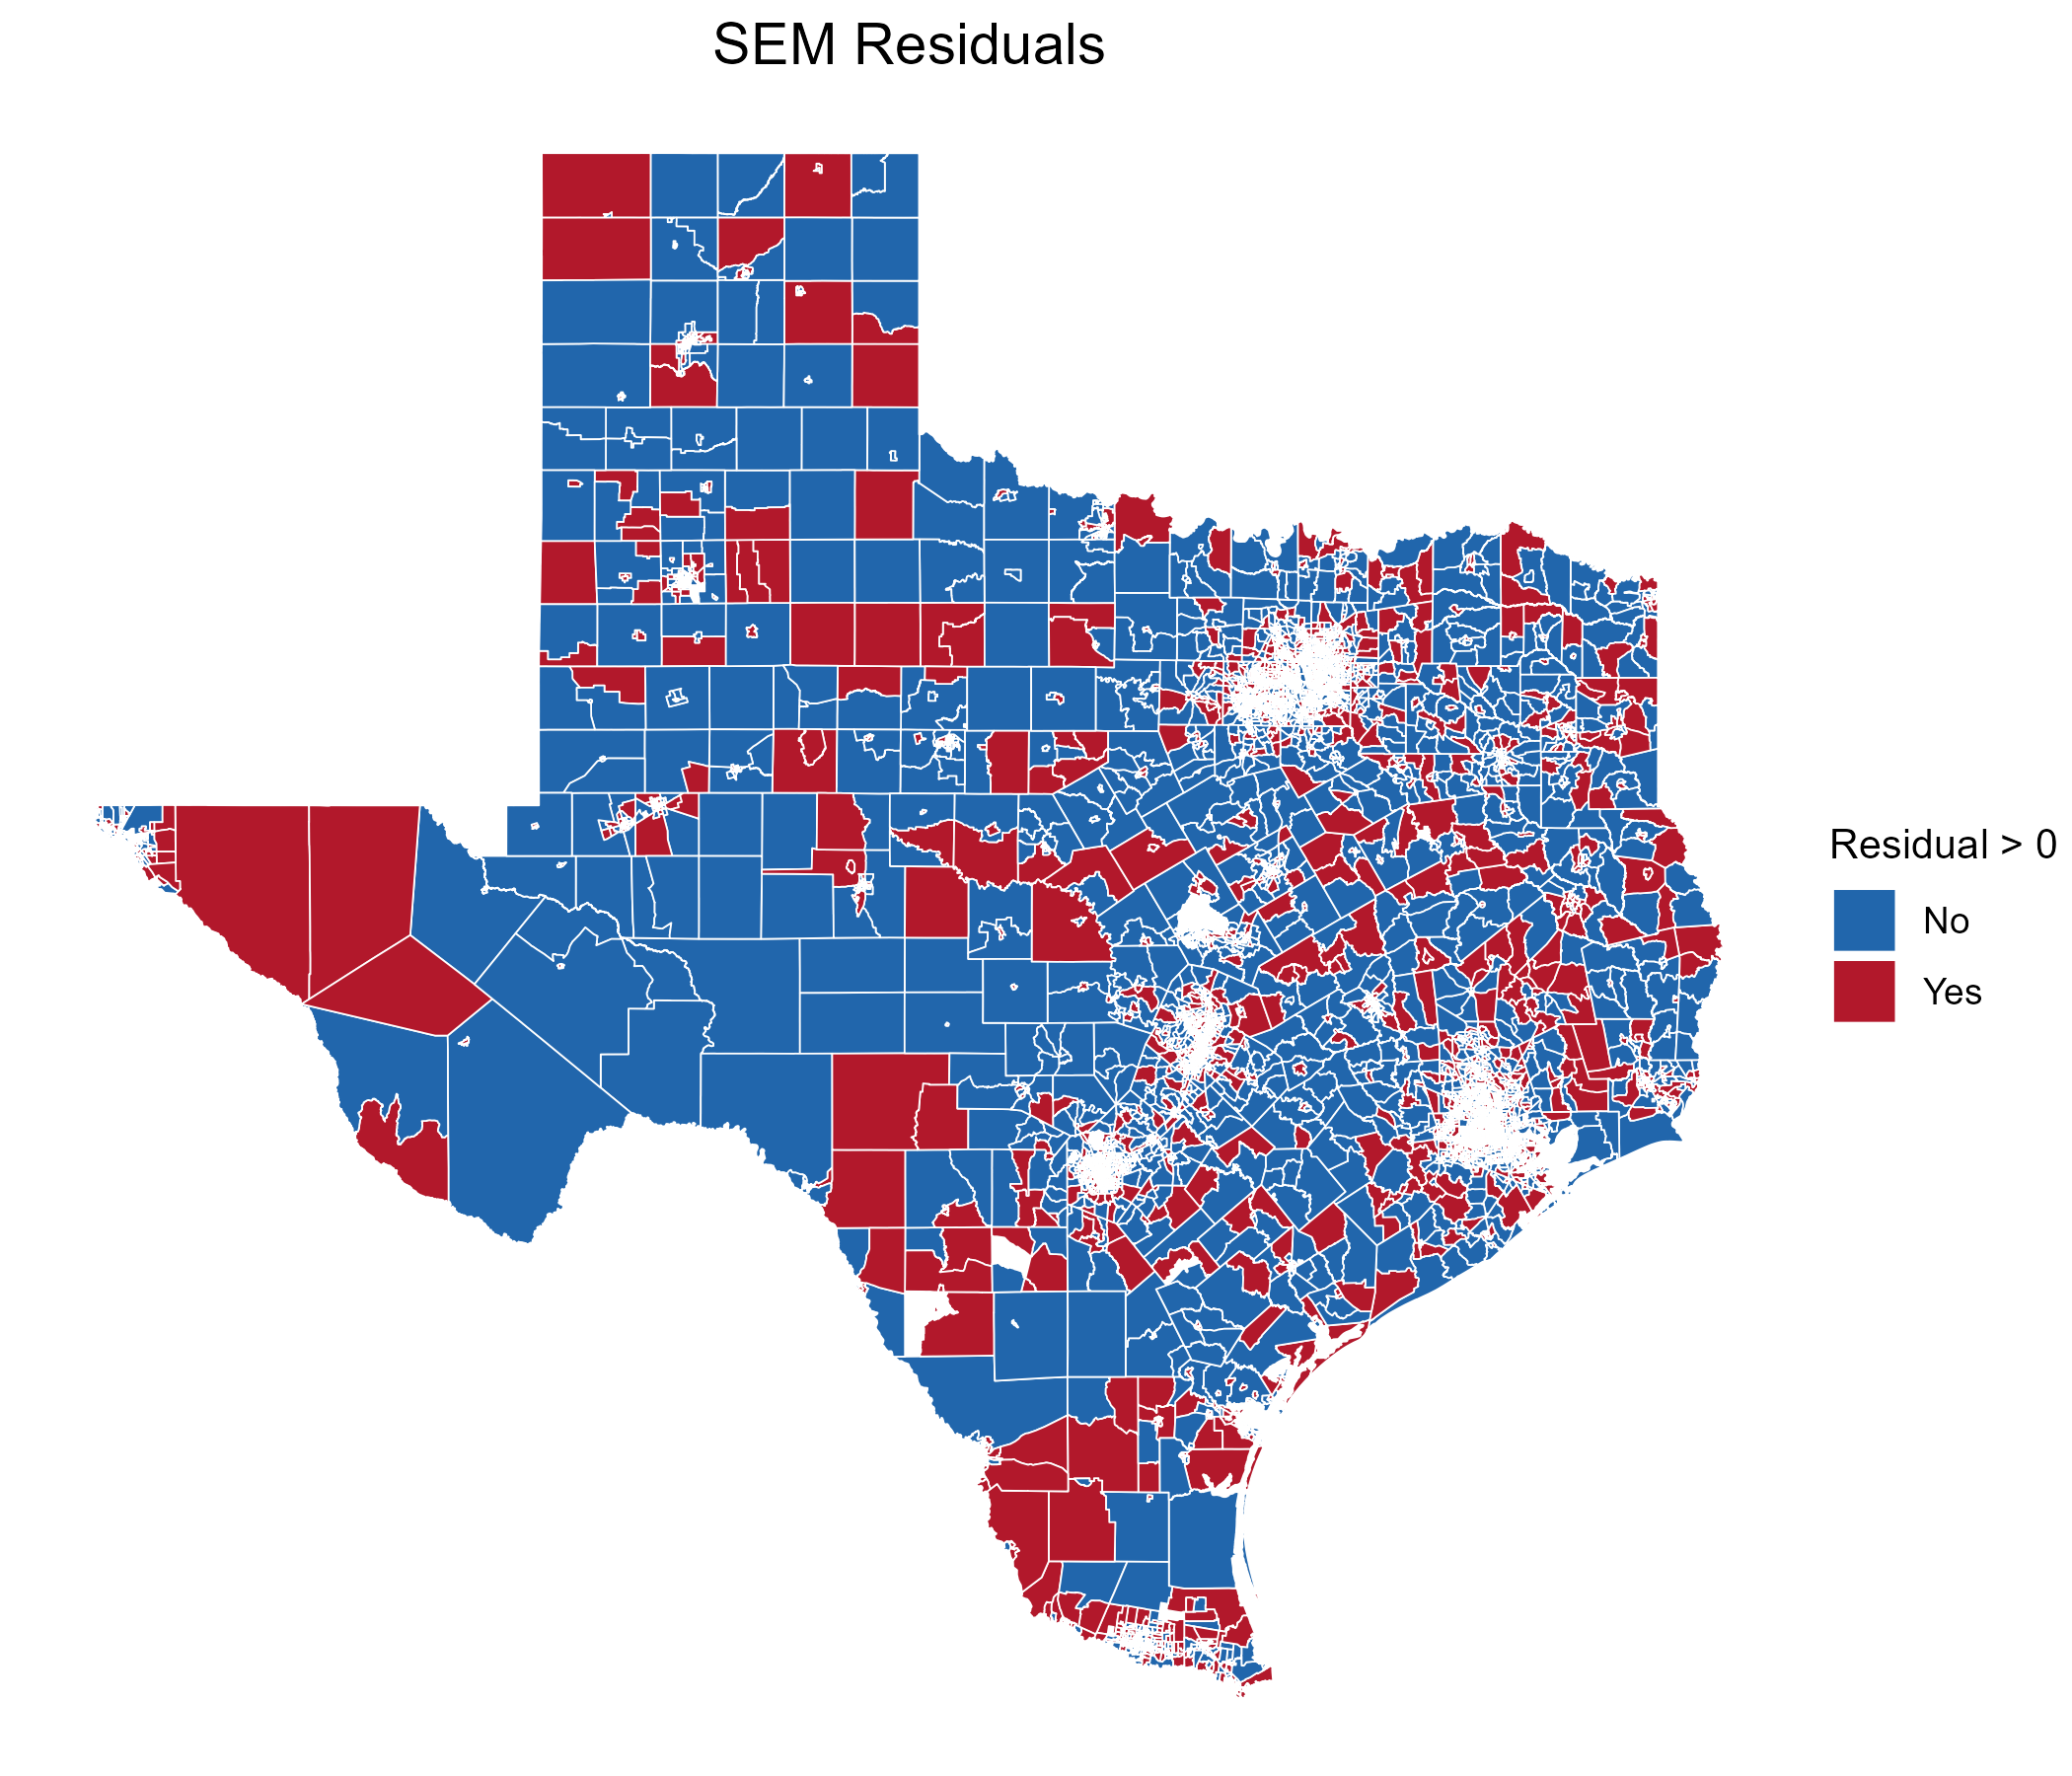
\includegraphics{sem_r_map.png}
\caption{Sem Map Res}
\end{figure}

\section{References}\label{references}

Beaulac, J., Kristjansson, E., \& Cummins, S. (2009). A systematic
review of food deserts, 1966--2007. \emph{Prevention of Chronic Disease,
6}, A105.
\url{https://resolver-scholarsportal-info.libaccess.lib.mcmaster.ca/resolve/15451151/v06i0003/nfp_asrofd1.xml}\\
Coleman-Jensen, A., Rabbitt, M. P., Gregory, C. A., \& Singh, A. (2019).
\emph{Household Food Security in the United States in 2018 (Economic
Research Report Number 270)}.
\url{https://doi.org/10.22004/ag.econ.301167}\\
Dean, W. R., \& Sharkey, J. R. (2011a). Food insecurity, social capital
and perceived personal disparity in a predominantly rural region of
Texas: An individual-level analysis. \emph{Social Science \& Medicine,
72(9)}, 1454--1462.
\url{https://doi.org/10.1016/j.socscimed.2011.03.015}\\
Dean, W. R., \& Sharkey, J. R. (2011b). Rural and urban differences in
the associations between characteristics of the community food
environment and fruit and vegetable intake. \emph{Journal of Nutrition
Education and Behavior, 43(6)}, 426--433.
\url{https://doi.org/10.1016/j.jneb.2010.07.001}\\
Government of Canada, S. C. (2023, November 14). \emph{Food insecurity
among Canadian families}.
\url{https://www150.statcan.gc.ca/n1/pub/75-006-x/2023001/article/00013-eng.htm}\\
Grummon, A. H., \& Taillie, L. S. (2018). Supplemental Nutrition
Assistance Program participation and racial/ethnic disparities in food
and beverage purchases. \emph{Public Health Nutrition, 21(18)},
3377--3385. \url{https://doi.org/10.1017/S1368980018002598}\\
Hernandez, D. C., Reesor, L. M., \& Murillo, R. (2017). Food insecurity
and adult overweight/obesity: Gender and race/ethnic disparities.
\emph{Appetite, 117}, 373--378.
\url{https://doi.org/10.1016/j.appet.2017.07.010}\\
Janda, K. (2020). \emph{A Geospatial Examination Of The Association
Between Geographic Food Access And Food Insecurity In Central Texas: The
Role Of Race/Ethnicity And Urbanicity} {[}Master's thesis, UTHealth
School of Public Health{]}. Dissertations \& Theses (Open Access).
\url{https://digitalcommons.library.tmc.edu/uthsph_dissertsopen/134}\\
Janda, K. M., Ranjit, N., Salvo, D., Hoelscher, D. M., Nielsen, A.,
Casnovsky, J., \& van den Berg, A. (2022). Examining geographic food
access, food insecurity, and urbanicity among diverse, low-income
participants in Austin, Texas. \emph{International Journal of
Environmental Research and Public Health, 19(9)}.
\url{https://doi.org/10.3390/ijerph19095108}\\
Lopez-Class, M., \& Hosler, A. S. (2010). Assessment of community food
resources: A Latino neighborhood study in upstate New York.
\emph{Journal of Poverty, 14(4)}, 369--381.
\url{https://doi.org/10.1080/10875549.2010.517070}\\
Myers, A. M., \& Painter, M. A. (2017). Food insecurity in the United
States of America: An examination of race/ethnicity and nativity.
\emph{Food Security, 9(6)}, 1419--1432.
\url{https://doi.org/10.1007/s12571-017-0733-8}\\
Nam, Y., Huang, J., Heflin, C., \& Sherraden, M. (2015). Racial and
ethnic disparities in food insufficiency: Evidence from a statewide
probability sample. \emph{Journal of the Society for Social Work and
Research, 6(2)}, 201--228.
\url{https://www.journals.uchicago.edu/doi/10.1086/681574}\\
Odoms-Young, A. M. (2018). Examining the impact of structural racism on
food insecurity: Implications for addressing racial/ethnic disparities.
\emph{Family \& Community Health, 41}(Suppl 2 FOOD INSECURITY AND
OBESITY), S3--S6. \url{https://doi.org/10.1097/FCH.0000000000000183}\\
Ramphul, R. (2020). \emph{Using Spatial Methods To Better Understand
Food Insecurity And Snap Under-Participation In Texas} {[}Master's
thesis, UTHealth School of Public Health{]}. Dissertations \& Theses
(Open Access).
\url{https://digitalcommons.library.tmc.edu/uthsph_dissertsopen/227}\\
Samuel, L. J., Crews, D. C., Swenor, B. K., et al.~(2023). Supplemental
Nutrition Assistance Program access and racial disparities in food
insecurity. \emph{JAMA Network Open, 6(6)}, e2320196.
\url{https://doi.org/10.1001/jamanetworkopen.2023.20196}\\
Walker, R. E., Keane, C. R., \& Burke, J. G. (2010). Disparities and
access to healthy food in the United States: A review of food deserts
literature. \emph{Health \& Place, 16(5)}, 876--884.
\url{https://doi.org/10.1016/j.healthplace.2010.04.013}

\end{document}
